\documentclass{amsart}
\title{The Projection-Ramification enumerative problem}
\usepackage{
  hyperref,
  amsmath,
  amssymb,
  amsthm,
  thmtools,
  microtype,
  stmaryrd,
  tikz,
  tikz-cd,
  todonotes,
  paralist
}

\ifcsname theorem\endcsname{}\else\declaretheorem[parent=section]{theorem}\fi
\ifcsname corollary\endcsname{}\else\declaretheorem[sibling=theorem]{corollary}\fi
\ifcsname lemma\endcsname{}\else\declaretheorem[sibling=theorem]{lemma}\fi
\ifcsname proposition\endcsname{}\else\declaretheorem[sibling=theorem]{proposition}\fi
\ifcsname conjecture\endcsname{}\else\declaretheorem[sibling=theorem]{conjecture}\fi
\ifcsname problem\endcsname{}\else\declaretheorem[sibling=theorem]{problem}\fi
\ifcsname question\endcsname{}\else\declaretheorem[sibling=theorem]{question}\fi
\ifcsname definition\endcsname{}\else\declaretheorem[sibling=theorem, style=definition]{definition}\fi
\ifcsname exercise\endcsname{}\else\declaretheorem[sibling=theorem, style=definition]{exercise}\fi
\ifcsname example\endcsname{}\else\declaretheorem[sibling=theorem, style=definition]{example}\fi
\ifcsname remark\endcsname{}\declaretheorem[sibling=theorem, style=remark]{remark}\fi


\providecommand {\N}{{\bf N}}
\providecommand {\Z}{{\bf Z}}
\providecommand {\Q}{{\bf Q}}
\providecommand {\R}{{\bf R}}
\providecommand {\C}{{\bf C}}

\renewcommand {\P}{{\bf P}}
\providecommand {\Gr}{{\bf Gr}}
\providecommand {\A}{{\bf A}}

\providecommand{\SL}{\operatorname{SL}}
\providecommand{\GL}{\operatorname{GL}}
\providecommand{\PGL}{\operatorname{PGL}}
\providecommand{\Gm}{{\bf G}_m}

\providecommand {\from}{{\colon}}

\providecommand{\spec}{\operatorname{Spec}}
\providecommand{\proj}{\operatorname{Proj}}
\providecommand{\coker}{\operatorname{coker}}
\providecommand{\Blowup}{\operatorname{Bl}}
\providecommand{\Hom}{\operatorname{Hom}}
\providecommand{\Ext}{\operatorname{Ext}}
\providecommand{\Tor}{\operatorname{Tor}}
\providecommand{\End}{\operatorname{End}}
\providecommand{\Aut}{\operatorname{Aut}}
\providecommand{\codim}{\operatorname{codim}}
\providecommand{\Pic}{\operatorname{Pic}}
\providecommand{\Sym}{\operatorname{Sym}}
\providecommand{\rk}{\operatorname{rk}} \declaretheorem[sibling=theorem, style=remark]{remark}
\declaretheorem[title=Theorem, style=plain]{maintheorem}
\renewcommand{\themaintheorem}{\Alph{maintheorem}}

\numberwithin{equation}{section}
\renewcommand{\k}{\mathbb{K}}
\DeclareMathOperator{\id}{id}
\DeclareMathOperator{\Bl}{Bl}
\DeclareMathOperator{\Hilb}{Hilb}
\DeclareMathOperator{\sing}{Sing}
\DeclareMathOperator{\F}{\mathbf F}
\DeclareMathOperator{\Ram}{Ram}
\DeclareMathOperator{\ord}{ord}
\newcommand{\Proj}{{\text{\rm Proj}\,}}
\renewcommand{\O}{\mathcal O}

\renewcommand{\sectionautorefname}{Section}
\renewcommand{\subsectionautorefname}{\S}
\renewcommand{\subsubsectionautorefname}{\S}


\begin{document}
\maketitle
 % (fold)
We calculate the degree of the projection-ramification map for as many varieties of minimal degree as we can.
After treating the relatively easy cases by hand, we relate the projection-ramification map for the Veronese surface and the quartic normal scroll with classical geometry of cubic plane curves.

\section{Rational normal curves}
\label{sec:arnc}
Let $X \subset \P^n$ be a rational normal curve.
Plainly, $X$ is incompressible, and hence the projection-ramification map
\[ \rho \from \Gr(2, n+1) \to \P^{2n-2}\]
is a regular map.
Therefore, we get
\begin{align*}
  \deg \rho &= c_1(\rho^* \O(1))^{2n-2}\\
            &= c_1(\O_{\Gr(r+1, n+1)}(1))^{2n-2} \\
            &= \frac{(2n-2)!}{n!(n-1)!}.
\end{align*}

\section{Quadric hypersurfaces} % (fold)
\label{sec:aquadricsurface}
A smooth quadric hypersurface $X \subset \P^{n}$ defined by a homogeneous quadric equation $F(X_{0},\dots,X_n) = 0$.
An easy calculation shows that the projection-ramification map
\[ \rho \from \P^n \to (\P^n)^*\]
is given in coordinates by
\[ p = [p_0: \dots:p_n] \mapsto \left[ \frac{\partial F}{\partial X_0}(p): \dots: \frac{\partial F}{\partial X_n}(p) \right].\]
In other words, it is the \emph{polarity isomorphism} induced by $F$, namely the isomorphism between a projective space and its dual given by the non-degenerate bilinear form associated to $F$.
In particular, we get $\deg \rho = 1$.

\section{The Veronese surface} % (fold)
\label{sec:veronese}
Let $\P^{2} \cong X \subset \P^{5}$ be the Veronese surface, the image of $\P^2$ under the complete linear series $\O(2)$.
In this case, the projection-ramification map
\begin{align*}
  \rho \from  \Gr(3,H^0(\P^2, \O(2))) \cong \Gr(3, 6) \dashrightarrow \P H^0(\P^2, \O(3))^* \cong \P^9
\end{align*}
can be described as follows.
Let $N \subset H^0(\P^2, \O(2))$ be a net of conics.
Then $\rho(N)$ corresponds to the cubic curve traced out by the nodes of the singular members of $N$, called the \emph{Jacobian} of $N$.
\begin{proposition}\label{prop:veronese}
  Let $R \subset \P^2$ be a general cubic.
  The fiber of $\rho$ over $[R]$ is in natural bijection with the set of non-trivial $2$-torsion line bundles on $R$.
  In particular, we have $\deg \rho = 3$.
\end{proposition}
The rest of \autoref{sec:veronese} is devoted to the proof of this assertion.

For the proof, we recall some classical projective geometry of cubics and nets of conics from \cite[\S~3]{dol:12}.
To distinguish the various copies of $\P^2$ that naturally arise in this story, write $\P^2 = \P V$ for a 3 dimensional vector space $V$.
Let $N \subset H^0(\P V, \O(2)) = \Sym^2V$ be a general net of conics on $\P V$.
Given a point $x \in \P N^*$, we denote the associated conic by $Q_x$.

There are three important cubic plane curves associated to the net $N$: the Jacobian curve, the discriminant curve, and the Hermite curve.
We have already seen the Jacobian curve $R \subset \P V$.
The \emph{discriminant curve} $D \subset \P N^*$ is the locus of $x \in \P N^*$ such that $Q_x$ is singular.
Since a pencil of conics contains three singular members, we see that $D$ is a cubic curve.
Note that if $Q_x$ is singular, then it is the union of two distinct lines in $\P V$.
A component line of $Q_x$ is called a \emph{Reye line}.
The \emph{Hermite curve} $E \subset \P V^*$ is the locus of Reye lines.
We leave it to the reader to check that it is a cubic curve.

The three cubic curves introduced above are inter-related.
First, we have an isomorphism $\tau \from D \to R$ defined by
\begin{equation}\label{eqn:DR}
  \tau \from x \mapsto \text{The singular point of $Q_x$}.
\end{equation}
Second, we have a degree 2 map $E \to D$ defined by
\[ \ell \mapsto \text{The $x \in D$ such that $Q_x$ contains $\ell$}.\]
Evidently, the fiber of this map over a given $x \in D$ corresponds to the two components of $Q_x$.
The (\'etale) degree 2 map $E \to D \cong R$ gives a non-trivial 2-torsion element $\eta \in \Pic(R)[2]$.
The element $\eta$ is characterized by the property that it is the unique non-trivial 2-torsion element whose pull-back to $E$ is trivial.

Denote by $H$ the hyperplane divisor class on $R \subset \P^2$.
\begin{lemma}\label{lem:reye}
  For every $a \in R$, the line joining $a$ and $a+\eta$ is a Reye line.
  Furthermore, this Reye line is a component of $Q_d$ where $d = \tau^{-1}(H-2a-\eta)$.
  Finally, the conjugate Reye line, namely the other component of $Q_d$, passes through the points $b$ and $b+\eta$ where $b \in R$ differs from $a$ by a non-trivial 2-torsion element other than $\eta$.
\end{lemma}
\begin{proof}
  Let $\ell$ be a general Reye line, and let $d \in D$ be such that $\ell$ is a component of $Q_d$.
  Let $x = \tau(d) \in R$ be the singular point of $Q_d$.
  Note that $\ell \cap R$ consists of three points, one of which is $x$.
  It suffices to show that the other two, say $y$ and $z$, differ by $\eta$.

  The point $y$ defines a line in $\P V^*$.
  This line intersects $E \subset \P V^*$ in three points, one of which is $\ell$, and the other two are the two components of $Q_{\tau^{-1}(y)}$; these correspond to the two pre-images of $y \in R$ under the double covering $E \to R$.
  Call these two points $y_1$ and $y_2$.
  Define $z_1$ and $z_2$ analogously.
  By construction, the triplets $y_1, y_2, \ell$ and $z_1, z_2, \ell$ are collinear triplets on $E \subset \P V^*$, and therefore we have the linear equivalence
  \[ y_1 + y_2 \sim z_1 + z_2\]
  on $E$.
  By pushing this forward to $R$, we get
  \[ 2y \sim 2z.\]
  Therefore, $y - z$ is a (non-trivial) 2-torsion element in $\Pic(R)$.
  However, the pull-back of $y-z$ is trivial on $E$, and hence $y - z = \eta$.

  Finally, let $m$ be the Reye line conjugate to $\ell$.
  Then it contains $x$, and two other points of $R$, say $y'$ and $z'$.
  By what we just proved, $y' - z' = \eta$.
  But we also have $y' + z' \sim y + z$.
  Hence $y - y'$ is a 2-torsion element, non-trivial, and distinct from $\eta$.
  The proof is now complete.  
\end{proof}

We now have all the tools to prove \autoref{prop:veronese}.
\begin{proof}[Proof of \autoref{prop:veronese}]
  Let $U \subset \P H^0(\P^2, \O(3))^*$ be the locus of smooth cubic curves, $J \to U$ be the universal Picard scheme, $J[2] \subset J$ the closed subscheme of 2-torsion classes, and $J[2]^* \subset J[2]$ the open and closed subscheme of non-trivial 2-torsion classes.
  The projection-ramification map for the Veronese surface factors as
  \begin{alignat*}{2}
    \rho \from \Gr(3, H^0(\P^2, \O(2))) &\dashrightarrow J[2]^* &&\dashrightarrow \P H^0(\P^2, \O(3))^*\\
    N &\mapsto (R, \eta) &&\mapsto R.
  \end{alignat*}
  We construct $J[2]^* \to \Gr(3,H^0(\P^2, \O(2)))$ inverse to the first map, which shows that $\deg \rho = 3$, and identifies the fibers of $\rho$ as non-trivial 2-torsion points.
  Given $(R, \eta) \in J[2]^*$, we need to construct a net $N$ of conics with Jacobian $R$.
  We use \autoref{lem:reye}, which tells us the singular elements of this net in terms of $R$ and $\eta$.
  Let $\{\eta, \eta', \eta''\}$ be the three non-trivial 2-torsion line bundles on $R$.
  Define the map $R \to \P H^0(\P^2, \O(2))^*$ by
  \[ R \ni a \mapsto \langle {a, a+\eta} \rangle \cup \langle {a+\eta', a+\eta''} \rangle ,\]
  where $\langle {p,q} \rangle$ denotes the line joining $p$ and $q$.
  We leave it to the reader to check that the image of $R$ is a plane cubic curve.
  The span of the image of $R$ is the desired net $N$.  
\end{proof}

\section{Quartic surface scroll}\label{sec:quartic_scroll}
Our next objective is to prove that $ \deg \rho_{X} = 2$ for a generic quartic surface scroll $X \subset \P^{5}$.
We begin by recasting $\rho_X$ in terms of nets of conics on $\P^2$, and bring in the projective geometry introduced in \autoref{sec:veronese}.

The generic quartic surface scroll $X \subset \P^5$ is isomorphic to $\P^1 \times \P^1$, embedded by the complete linear system associated to $\O(1,2)$.
Say $\P^1 \times \P^1 = \P U \times \P V$, where $U$ and $V$ are two-dimensional vector spaces.
Then the projection-ramification map is a $\PGL(U) \times \PGL(V)$-equivariant map
\[
  \Gr(3, U \otimes \Sym^2 V) \dashrightarrow \P(U \otimes \Sym^4 V)^*.
\]
We take the quotient of both sides by the $\PGL(U) \times \PGL(V)$-action.
We begin by identifying the two quotients.

Let $S$ be a 3-dimensional quadratic space, that is, a vector space with a non-degenerate quadratic form $q$.
Then we have $\Aut(S) =  \operatorname{O}(q) \cong \operatorname{O(3)}$.
The projective space $\P S$ is isomorphic to $\P^2$, and it comes with a distinguished smooth conic $Q \subset \P S$.
The automorphism group of the pair $(\P S, Q)$ is $\Aut(Q) \cong \PGL_2$.
\begin{lemma}\label{lem:quotgrass}
  The quotient $\Gr(3, U \otimes \Sym^2V) / \PGL(U) \times \PGL(V)$ is birational to the quotient $\Hilb^3(\P S) / \Aut S$.
\end{lemma}
\begin{proof}
  Let $W$ be a 3-dimensional vector space.
  We have a birational isomorphism
  \begin{align*}
    \Gr(3, &U \otimes \Sym^3 V) / \PGL(U) \times \PGL(V)\\
           &\sim (W^* \otimes U \otimes \Sym^2 V) / \GL(W) \times \GL(U) \times \GL(V).
  \end{align*}
  Interpret the space $(W^* \otimes U \otimes \Sym^2 V) / \GL(W) \times \GL(U)$ as the space of $2 \times 3$ matrices with entries in $\Sym^2 V$, modulo row and column transformations.
  Set $S = \Sym^2 V$; it has a canonical (up to scaling) quadratic form given by the conic $Q \cong \P V\subset \P S$ embedded by $\O(2)$.
  We can then interpret $(W^* \otimes U \otimes \Sym^2 V) / \GL(W) \times \GL(U)$ as the space of $2 \times 3$ matrices with entries in $S$.
  We have a rational map
  \begin{align*}
    (W^* \otimes U \otimes \Sym^2 V) / \GL(W) \times \GL(U) &\dashrightarrow
                                                              \Hilb^3(\P S) \\
    \text{$2 \times 3$ matrix $M$} &\mapsto \text{Vanishing locus of $2\times 2$ minors of $M$}.
  \end{align*}
  It is easy to check that this map is a birational isomorphism---a general triple of points in $\P S$ is the zero locus of $2 \times 2$ minors of a $2 \times 3$ matrix of linear forms, which is uniquely determined up to row and column transformations.
  By taking a further quotient by $\GL(V)$, we finish the proof.  
\end{proof}

\begin{lemma}\label{lem:quotram}
  The quotient $\P(U \otimes \Sym^4 V)^* / \PGL(U) \times \PGL(V)$ is birational to the quotient $\Gr(2, (\Sym^2 S)/q) / \Aut S$.
\end{lemma}
\begin{proof}
  We have the birational isomorphism
  \begin{align*}
    (U \otimes \Sym^4 V) / \GL(U) &\sim \Gr(2, \Sym^4 V).
  \end{align*}
  Note that $q \in \Sym^2S$ spans the kernel of the natural surjection $\pi \from \Sym^2 S \to \Sym^4 V$.
  So the claimed birational isomorphism is given by sending a two dimensional subspace $L \subset \Sym^4 V$ to the image of $\pi^{-1}L$ in $\Sym^2S/q$.
\end{proof}

Via the birational isomorphisms in \autoref{lem:quotgrass} and \autoref{lem:quotram}, the projection-ramification map $\rho_X$ transforms into an $\Aut(S)$-equivariant map
\[
  \mu \from \Hilb^3\P S \dashrightarrow \Gr(2, \Sym^2S/q).
\]
We now describe this map $\mu$ explicitly.
To ease notation, we denote a linear form and its vanishing locus by the same letter.
Let $\xi \in \Hilb^3 \P S$ be a general point corresponding to the three vertices of the triangle formed by three lines $L_i$ for $i = 1, 2, 3$.
Restricting the two lines $L_i$ and $L_j$ to $Q$ gives two quadratic forms $L_i|_Q$ and $L_j|_Q$ on $Q$.
Let $R_{ij}$ be the line whose intersection with $Q$ is the ramification divisor of the pencil $\langle  L_i|_Q, L_j|_Q \rangle$.
It is easy to check that the quadrics $L_1 R_{23}$, $L_2 R_{13}$, and $L_3R_{12}$ span a 3-dimensional subspace of $\Sym^2 S$ that contains the quadric $q$.
\begin{lemma}\label{lem:mu}
  In the setup above, the image of $\xi$ under $\mu$ is the image of $\langle  L_1R_{23}, L_2R_{13},L_3R_{12} \rangle$ in $\Sym^2S/q$.
\end{lemma}
\begin{proof}
  The ideal of the point $\xi \in \Hilb^3(S)$ is cut out by the $2 \times 3$ matrix of linear forms
  \[
    M =
    \begin{pmatrix}
      L_1 & 0 & L_3 \\
      0 & L_2 & L_3
    \end{pmatrix}.
  \]
  Let $U_0, U_1$ be a basis of $U$.
  Under the isomorphism in \autoref{lem:quotgrass}, this $2 \times 3$ matrix corresponds to the point of $\Gr(3, U \otimes \Sym^2 V)$ given by the subspace of $U \otimes \Sym^2 V$ spanned by $U_0 M_{0,i} + U_1 M_{1,i}$ for $i = 1, 2, 3$.
  From \eqref{eqn:Rmatrix}, the ramification divisor of this subspace is given by
  \begin{align*}
    R &= \det
    \begin{pmatrix}
      L_1 & 0 & U_0 L_1' \\
      0 & L_2 & U_1 L_2' \\
      L_3 & L_3 & (U_0+U_1)L_3'
    \end{pmatrix} \\
      &= U_0L_2(L_3'L_1 - L_1L_3') + U_1L_1(L_3'L_2-L_2L_3')\\
      &= U_0L_2R_{13} + U_1 L_1R_{23}.
  \end{align*}
  In this calculation, $L_i'$ denotes the derivative $\frac{d}{dt}$ of $L_i$ considered as an element of $\k[t]$ by pullback under some parametrization $\spec \k[t] \to Q$ and trivialization of $\O(2)|_{\spec \k[t]}$.
  Although the derivative depends on the choices, the forms $L_iL_j' - L_jL_i'$ do not, and they cut out precisely the ramification divisor of the pencil $\langle  L_i|_Q, L_j|_Q \rangle$.
  Under the isomorphism in \eqref{lem:quotram}, the divisor $R$ corresponds to the 2 dimensional subspace of $\Sym^2 S/q$ spanned by $L_2R_{13}$ and $L_1R_{23}$ (The roles of $L_1, L_2, L_3$ can be changed by linear transformations of $M$, so we get that $L_3R_{12}$ also lies in this span).
  The proof is thus complete.
\end{proof}

Recall that the conic $Q \subset \P S$ gives an isomorphism $\P S \cong \P S^*$, called \emph{polarity} with respect to $Q$.
On the vector spaces, it is the isomorphism induced by the bilinear form associated to $q$.
Geometrically, it is characterized by the rule that the polar of a point $p \in Q$ is the tangent line to $Q$ at $p$.
More generally, given a point $p \in \P S$, the pencil of lines through $p$ contains two lines tangent to $Q$; the polar of $p$ is the line joining the two points of tangency.
We denote the polar of a point $p$ (resp. a line $L$) by $p^\perp$ (resp. $L^\perp$).

Set $M_i = R_{jk}$, and let $N$ be the net spanned by $L_iM_i$ for $i = 1, 2, 3$.
By the definition of $R_{jk}$, we see that $M_i$ is the polar line of the point $L_j \cap L_k$.
In other words, the triangles $(L_1, L_2, L_3)$ and $(M_1, M_2, M_3)$ are polar conjugates---lines in one are polars to the vertices of the other (see \cite[\S~2.1.4]{dol:12}).

\begin{remark}[This long remark is only for context, and is not logically necessary for what comes next]
  \label{rem:richelot}
  The space $\Hilb^3 \P S / \Aut S$ and its birational involution (called the Richelot involution) induced by
  \begin{equation}\label{eqn:richelot}
    \tau \from \Hilb^3 \P S \dashrightarrow \Hilb^3 \P S
  \end{equation}
  that sends a triangle formed by the lines $(\ell_1, \ell_2, \ell_3)$ to the triangle formed by the points $(\ell_1^\perp, \ell_2^\perp, \ell_3^\perp)$ have well-known moduli interpretations, which we learned from \cite[Example~4.2]{dol.how:15}.
  Intersecting the lines $\ell_i$ with $Q$ for $i = 1, 2, 3$ gives a triple of pairs of points on $Q \cong \P^1$.
  The double cover of $\P^1$ branched along these six points gives a genus 2 curve $C$.
  The grouping of the six points in three pairs $\{p_i, q_i\}$ for $i = 1, 2, 3$ gives a 2-dimensional subspace of the 4-dimensional $\F_2$-vector space $\Pic C [2]$, namely $\{0\} \cup \{p_i - q_i \mid i = 1,2,3\}$.
  This vector space is a maximal isotropic subspace for the Weil pairing on $\Pic C[2]$.
  Conversely, a genus 2 curve $C$ with a maximal isotropic subspace of $\Pic C[2]$ defines six points on $\P^1$ grouped into a triple of pairs.
  Thus, $\Hilb^3 \P S / \Aut S$ is birational to the moduli space of genus 2 curves along with an isotropic subspace of 2-torsion points in its Jacobian.

  Since general principally polarized abelian surfaces are Jacobians of genus 2 curves, $\Hilb^3 \P S / \Aut S$ is also birational to the moduli of $(A, G)$, where $A$ is a principally polarized abelian surface and $G \subset A[2]$ is a maximal isotropic subspace for the Weil pairing.
  In this interpretation, the involution $\tau$ is called the Fricke involution; it sends $(A, G)$ to $(A/G, A[2]/G)$ (see \cite[Page~2]{muk:12}).

  Using the Torelli theorem, the moduli space of $(A, G)$ can be described as the quotient $H_2/\Gamma_0(2)$, where $H_2$ is the Siegel upper half space of degree 2, and $\Gamma_0(2) \subset \operatorname{Sp}(4, \Z)$ is the congruence subgroup consisting of matrices $\begin{pmatrix} A & B \\ C & D \end{pmatrix}$ where $A, B, C, D$ are $2 \times 2$ blocks and $C \equiv 0 \pmod 2$.
  In this interpretation, the involution $\tau$ is induced by the action of $\frac{1}{\sqrt 2} \begin{pmatrix} 0 & I_2 \\ -2 I_2 & 0 \end{pmatrix} \in \operatorname{Sp}(4, \R)$ on $H_2$ (again, see \cite[Page~2]{muk:12}).

  Finally, suppose we pass to ordered triples of pairs, or equivalently to $(\P S)^3 / \Aut S$.
  Then the moduli interpretation changes slightly.
  Now the space is the moduli space of $(A, \psi)$, where $A$ is a principally polarized abelian surface and $\psi \from \F_2^2 \to A[2]$ is an isomorphism onto a maximal isotropic subspace (note that $\psi$ is equivalent to a maximal isotropic $G \subset A[2]$ along with a basis of $G$).
  The moduli space of $(A, \psi)$ is the quotient $H_2 / \Gamma_1(2)$ where $\Gamma_1(2) \subset \operatorname{Sp}(4, \Z)$ is defined by the congruence conditions $A - I_2 \equiv 0 \pmod 2$ in addition to $C \equiv 0 \pmod 2$.
  The Fricke involution continues to act on $H_2 / \Gamma_1(2)$.
  The Satake compactification of $H_2 / \Gamma_1(2)$ is the Igusa quartic threefold in $\P^4$ on which the Fricke involution acts by a linear transformation of $\P^4$.
  The quotient of the Igusa quartic by the Fricke involution is isomorphic to a double cover of $\P^3$ branched along the union of 4 planes  \cite[Theorem~2]{muk:12}.
  \qed
\end{remark}

Recall that $\xi \in \Hilb^3\P S$ is the point defined by the three vertices of the triangle formed by $(L_1, L_2, L_3)$.
Let $\xi' \in \Hilb^3\P S$ be the point defined by the three vertices of the triangle formed by $(M_1, M_2, M_3)$.
\begin{proposition}\label{prop:quarticscroll}
  In the setup above, $\xi$ and $\xi'$ are the only points of $\Hilb^3\P S$ that map to $N \in \Gr(2, \Sym^2S/q)$.
  In particular, the degree of $\mu \from \Hilb^3\P S \dashrightarrow \Gr(2, \Sym^2S/q)$ is 2.
\end{proposition}
We invite the reader to look at \autoref{fig:quarticscroll} for the configuration formed by the conic $Q$, the Jacobian $R$, the polar of the Hermite curve $E^\perp$, and the triangles $(L_1,L_2,L_3)$ and $(M_1,M_2,M_3)$.
\begin{proof}
  By \autoref{lem:mu}, we see immediately that $\mu(\xi') = \mu(\xi) = N$.
  To show that no other triangles map to $N$, consider pairs of triplets $\Delta = (\Delta_1, \Delta_2, \Delta_3)$ and $\nabla = (\nabla_1, \nabla_2, \nabla_3)$ of lines in $\P S$ such that
  \begin{enumerate}
  \item $\Delta$ and $\nabla$ are polar conjugates with respect to $Q$, and
  \item $\Delta_i \cup \nabla_i$ is an element of $N$ for $i = 1, 2, 3$.
  \end{enumerate}
  It suffices to show that the only ones satisfying the two conditions are $(L_1, L_2, L_3)$ and $(M_1, M_2, M_3)$, up to permutation.
  
  To show this, we need some observations.

  First, suppose $A_1 \cup B_1$ and $A_2\cup B_2$ are elements of the net $N$, where $A_i$ and $B_j$ are lines in $\P S$.
  Then, by definition, $A_i$ and $B_j$ are Reye lines of the net $N$.
  Let $p = A_1 \cap A_2$ and $t = B_1 \cap B_2$.
  We claim that the third Reye line through $p$, in addition to $A_1$ and $A_2$, is the line $\langle p, t\rangle$.
  To see this, note that in the pencil of conics spanned by $A_1 \cup B_1$ and $A_2 \cup B_2$, the third singular conic is $\langle p, t\rangle \cup \langle p', t'\rangle$, where $p' = A_1 \cap B_2$ and $t' = A_2 \cap B_1$.

  Second, let $R \subset \P S$ be the Jacobian cubic and $E \subset \P S^*$ be the Hermite cubic of $N$.
  Let $E^\perp \subset \P S$ be the image of $E$ under the polarity isomorphism $\P S^* \to \P S$ induced by $Q$.
  Explicitly, the points of $E^\perp$ are the polars of the Reye lines.
  We claim that the six points of intersection of $R$ and $Q$ also lie on $E^\perp$.
  Indeed, to show that $x \in R \cap Q$ also lies on $E^\perp$, it suffices to show that the line $T_xQ$ is a Reye line.
  Since $x \in R$, there exists an element of $N$ of the form $A\cup B$ where $A$ and $B$ are lines intersecting at $x$.
  Note that in the pencil of conics spanned by $A \cup B$ and $Q$, there is a singular conic containing $T_xQ$.
  Therefore, $T_xQ$ is a Reye line.
  
  Third, since $R \cap E^\perp$ contains 6 points on the conic $Q$, the residual 3 points are collinear.
  Let them correspond to $x_1, x_2, x_3 \in E$.
  Denoting by $H$ the hyperplane class of $E \subset \P S^*$, we have the equation in $\Pic E$
  \[ x_1 + x_2 + x_3 = H.\]

  Having made the three necessary observations, we resume the proof.
  Suppose we have two triangles $\Delta$ and $\nabla$ satisfying the two conditions above.
  Consider the point $p_3 = \Delta_3 \cap \nabla_3$.
  By the second condition, it lies on $R$.
  By the polar conjugacy of $\Delta$ and $\nabla$, we have
  \begin{align*}
    p_3^\perp &= \langle \Delta_3^\perp, \nabla_3^\perp \rangle \\
              &= \langle  \nabla_1 \cap \nabla_2, \Delta_1 \cap \Delta_2\rangle.
  \end{align*}
  By the first observation, we see that $p_3^\perp$ is a Reye line.
  Hence $p_3$ lies on $E^\perp$, and hence on $R \cap E^\perp$.
  Similarly, $p_1 = \Delta_1 \cap \nabla_1$ and $p_2 = \Delta_2 \cap \nabla_2$ also lie on $E^\perp$.
  Since $N$ is general, we may assume that the $p_i$ do not lie on $Q$.
  Hence, $p_1, p_2, p_3$ are the three collinear points in $R \cap E^\perp$.
  (The fact that $p_1, p_2, p_3$ are collinear is not surprising---it is because any two polar conjugate triangles are in linear perspective \cite[Theorem~2.1.9]{dol:12}).
  By reordering if necessary, assume that we have $p_i^\perp = x_i$ as elements of $E$.

  Now, observe that the three Reye lines through the vertex $\Delta_1 \cap \Delta_2$ are $\Delta_1$, $\Delta_2$, and $p_3^\perp$, and likewise for the other two vertices.
  The concurrence of the three lines, along with the equality $p_3^\perp = x_3$, yields the system of equations on $\Pic E$
  \begin{align*}
    \Delta_1 + \Delta_2 + x_3 &= H, \\
    \Delta_2 + \Delta_3 + x_1 &= H, \\
    \Delta_3 + \Delta_1 + x_2 &= H. \\
  \end{align*}
  Of course, the same three equations hold if we replace $\Delta$ by $\nabla$.

  Note that the points $x_1, x_2, x_3 \in E$ are determined by $N$.
  Using $x_1 + x_2 + x_3 = H$, a simple calculation gives $2 \Delta_1 = 2x_1$.
  This equation has 4 solutions for $\Delta_1$, namely $x_1 + \epsilon$ for $\epsilon \in \Pic E[2]$.
  Also, $\Delta_1$ determines $\Delta_2$ and $\Delta_3$ by the equations above, which in turn determine the $\nabla_i$ using polarity or the property that $\nabla_i$ and $\Delta_i$ form a fiber of the map $E \to R$.
  Thus, it suffices to show that at most two of the four solutions for $\Delta_1$ can be valid.

  Suppose $\Delta_1 = x_1$.
  Then we get $\Delta_2 = x_2$, and $\Delta_3 = x_3$.
  However, the lines represented by the $x_i$ are concurrent, whereas the lines $\Delta_i$ are not.
  Therefore, we get that $\Delta_1 \neq x_1$.
  The same argument shows that $\nabla_1 \neq x_1$.
  Let the involution of $E$ induced by $E \to R$ be given by the addition of $\epsilon_0 \in \Pic E [2]^*$.
  Since $\Delta_1$ and $\nabla_1$ form a fiber of $E \to R$, we have $\nabla_1 = \Delta_1 + \epsilon_0$.
  So, $\nabla_1 \neq x_1$ translates into $\Delta_1 \neq x_1 + \epsilon_0$.
  In summary, the only two possible solutions for $\Delta_1$ are $x_1 + \epsilon$ for $\epsilon \in \Pic E [2] \setminus \{0, \epsilon_0\}$.
  The proof is now complete.  
\end{proof}
\vfill
\begin{figure}
  \centering
  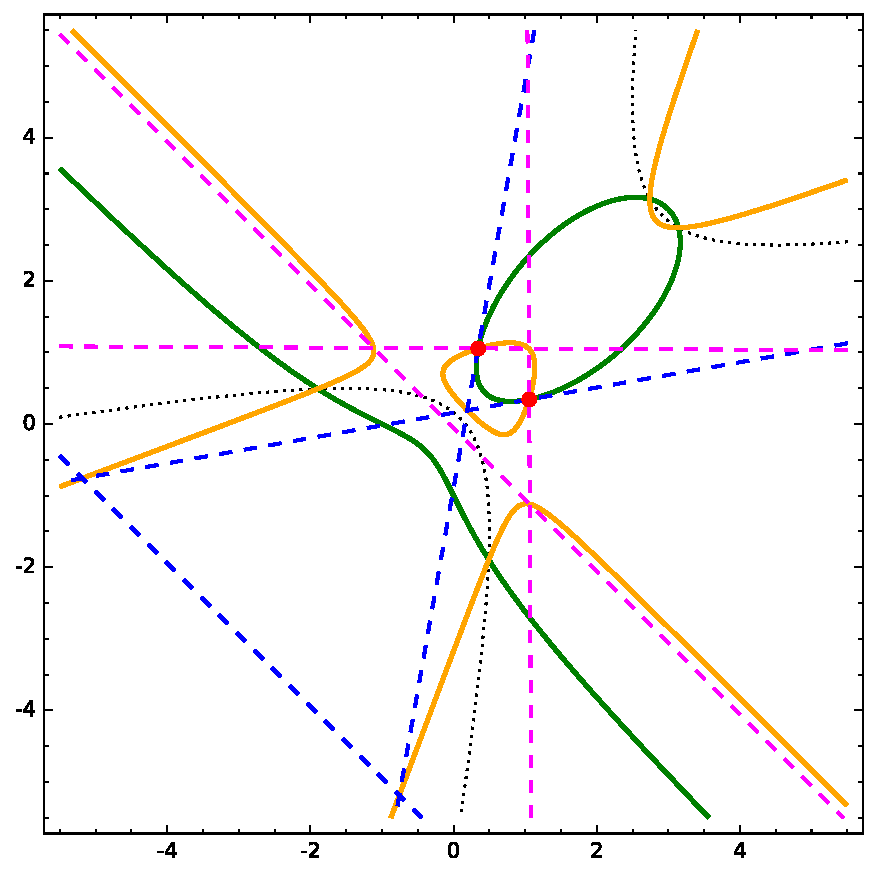
\includegraphics{quartic_scroll}
  %The smiling octopus.
  \caption{
    The figure shows the unique pair of polar conjugate triangles of Reye lines associated to a net of conics as proved in \autoref{prop:quarticscroll}.
    The net includes the distinguished conic $Q$, seen here as a hyperbola (dotted black).
    The Jacobian cubic $R$ (green) and the dual of the Hermite cubic $E^\perp$ (orange) intersect in 6 points on $Q$ (4 of which are real and visible), and 3 other collinear points, two of which, say $p_1$ and $p_2$, are marked (red), and the third, say $p_3$, is at infinity.
    The Reye lines forming the two polar conjugate triangles (dashed pink and dashed blue) come in conjugate pairs.
    The lines in each pair intersect at $p_1$, $p_2$, and $p_3$.
    (The figure was produced using \texttt{Sage} \cite{the:17}.)
  }
  \label{fig:quarticscroll}
\end{figure}
\end{document}
